\begin{figure}[h]
	\centering
	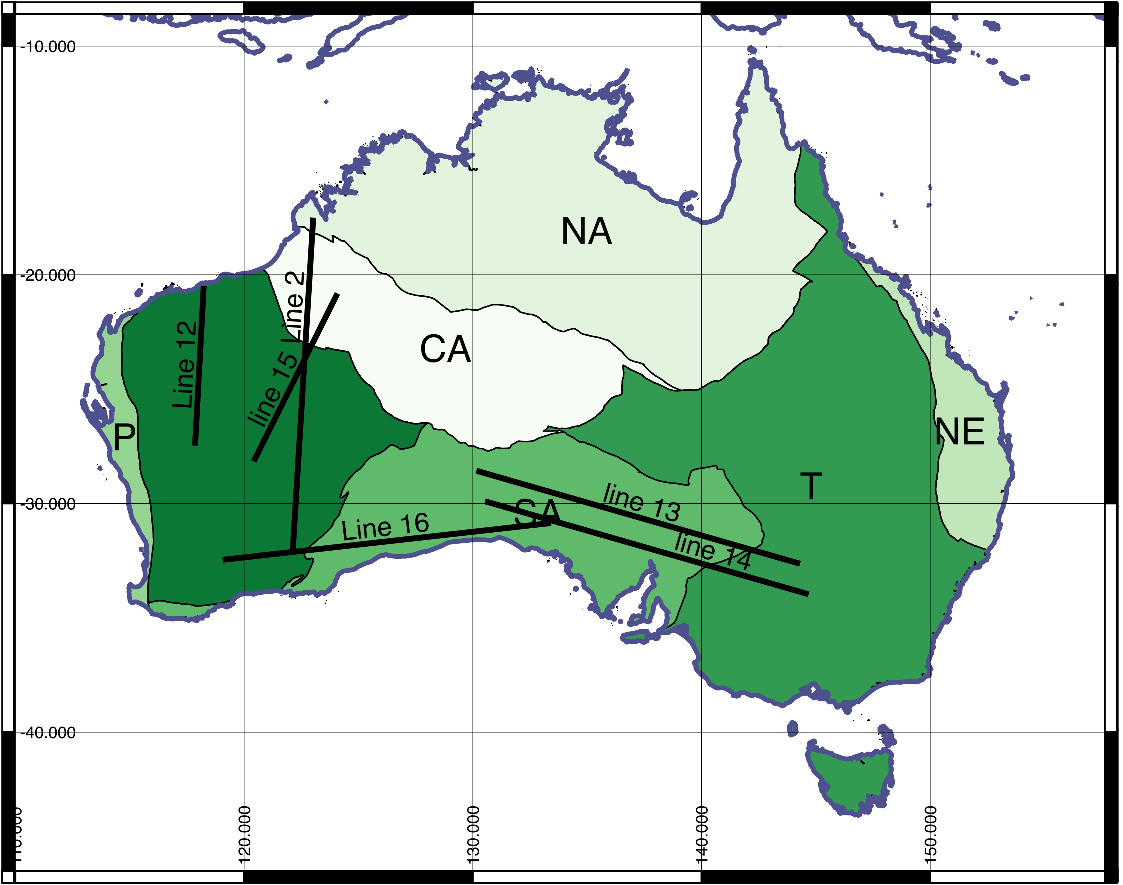
\includegraphics[width=1\linewidth]{../fig/maps/aus_lines}
	\caption[Australian lines]{Australian lines used to detect change points in this study. The polygons refers to  mayor Australian crustal elements.}
	\label{fig:aus_lines}
\end{figure}

\section{Work flow}
So far I've been using data from Geoscience Australia (Gravity 900m grid, magnetic 90m grid, and radiometric (K, Th and U, 100m grid), GOCE (gravity, 37km grid) and ADMAP (magnetic, 5km grid, in best cases). I don't have the exact reference for the data sets as they have been changing hands a few times before I got it. 

I use a GIS software (QGIS) to locate lines and sample raster vales along lines. It's fairly easy to select lines and they don't need to be straight, in case a curved line would better capture an expected boundary. The choice of lines have been discussed with Dr Jacqueline Halpin and Dr. Joanne Whittaker. When the technique is working, longer lines would be more useful.

During coding and evaluation, I've only been working on a few datasets, mainly Line 12 and 15, however, for this report I applied the method to a number of lines to guide further work: 

\begin{itemize}
	\item [2] From North to south from Kimberley into Yilgarn. 
	\item [12] Pilbara into Yilgarn.
	\item [13] Across Gawler North.
	\item [14] Across Gawler South (for reference to compare with \textit{Line 13}).
	\item [15] As 2, but perpendicular to suggested boundaries.
	\item[16] From Yilgarn, accross Albany Fraser into central South Australia. 
\end{itemize}

To shorten the processing time and to adjust resolution, the time-series are sub sampled [see figures]. Typically, when testing the code I'll sub-sample the resolution down to $1:100$, 10km, but later run typically $1:5$, 500m sampling distance. Sub-sampling is performed by applying a rolling average (essentially a LP filter) with the same window length as the sub-sampling, e.g. 5 samples. From the smoothed dataset, I pick every $n$th sample (\texttt{data[::n]}). 

The units of the data, naturally, varies in a large range and as I'm not interested in the actual data [sic] but rather the statistical changes in it. Therefore the individual datasets are normalised to a fixed range ($0-1$). 

An important watershed in change detection, is between \textit{on-line } and  \textit{off-line} methods. The first have the obvious advantage of detecting change in a stream of data, and is therefore optimized for minimal time delay. The Bayesian and Markov-chain approach works by looking at the running partition with increased scepticism but also to estimate the prior. 

I'm using a Python script to run the change-point detection. The speed depends on the square of the amount of data. That is the resolution of sample-points along lines, lengths of lines, layers of data for multivariate detection. Typically calculation time is less than one minute for a line with samples down-sampled to 1km resolution. On-line algorithm is faster than the off-line approach. Methods to speed up off-line calculations have been suggested by e.g. Xuan and Murphy \cite{Xuan2007}. There is still room for improvements in my code. 


\begin{figure}[h]
	\centering
	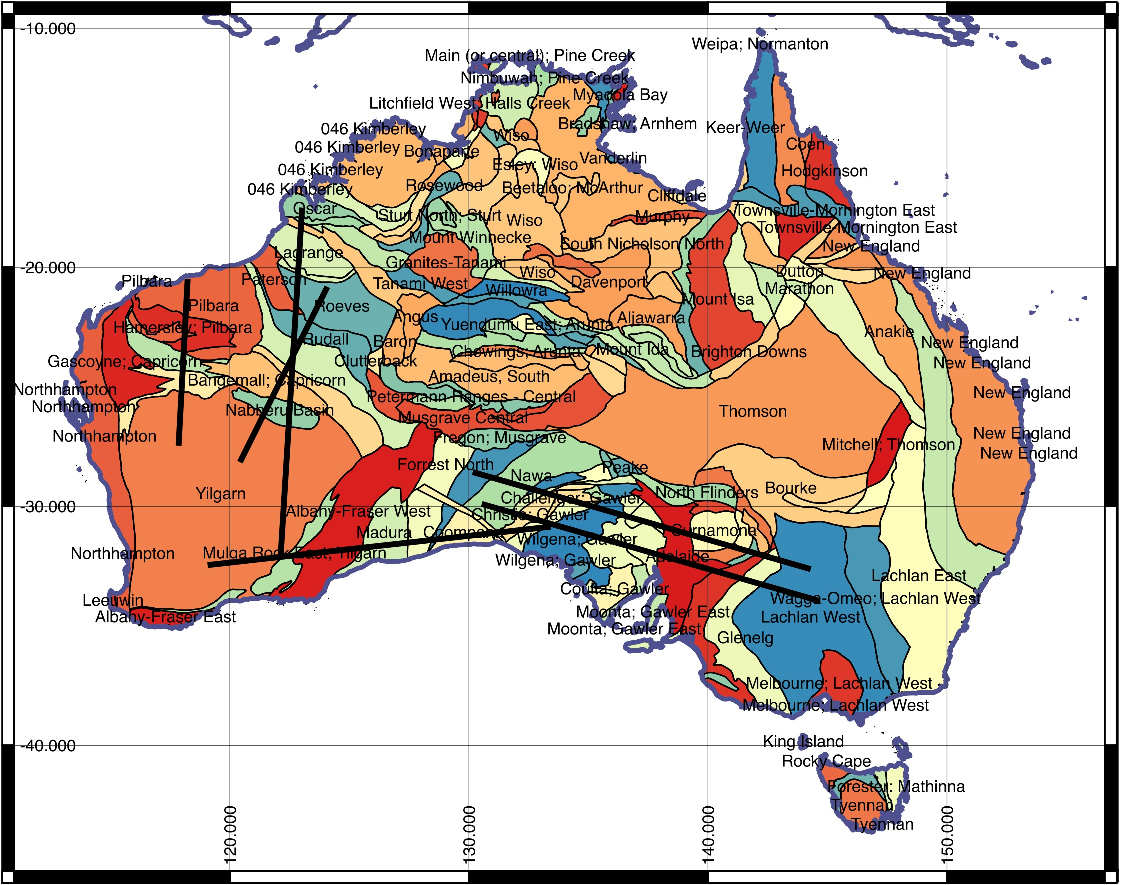
\includegraphics[width=1\linewidth]{../fig/maps/aus_geo}
	\caption[Australian geology]{The geology of Australia. The color map is trivial. These boundaries are plotted with change-points in the figures.}
	\label{fig:aus_geo}
\end{figure}



\section{Naïve techniques}
To get a first estimate of the prior function, I've been looking at the time series and calculated mean and variance over time (also known as rolling mean and roiling variance). In this example I show how average and variance of the data in 1D suggests boundaries. I also calculate the derivative of the rolling average and variance as it is the change of states I am interested in. With a number of parameters, the figures easily get clogged, but the average of the parameters gives an indication of the trends. To be useful, a weighting should be applied to the average. 

The \textit{naïve} plots are used as a reference to suggest to origin of detected change points. 

\section{On-line techniques}
I've been trying on-line techniques as they are very fast. However, there is little benefit in this application, as we know the data for the whole extension of the lines. I did not manage to create a multivariate on-line change-point detection, but that should be possible with a covariance estimate. 1-parameter off-line results are very similar to the on-line plots showed here \cite{Adams2007}. 



\section{Off-line techniques}
Off-line change-point detection would look at the whole line and use a Bayesian approach as suggested by Fearnhead \cite{Fearnhead2006} and developed by Xuan to use covariance models for multivarate data \cite{Xuan2007}. The method works well for datasets with an unknown number of change-points.
I'm using a full covariance model that have the advantage over an naïve independent features model as I expect parameters variance and mean to be linked through an unknown function rather than completely independent. Xuan and Murphy suggest a faster Gaussian graphical model that is supposed to give similar results but is much faster and might have other advantages in higher dimensions. I did not try the function yet, and it might not  be so interesting as I'll probably only use 2-4 datasets in the Antarctic application anyway. 

%\subsection{Gauss vs Xuan}


